
\section*{Background Knowledge}

\subsection*{
    GAN
}
The GAN architecture consist of two principal component :
Generator (G) and Discriminator (D) .
The main goal of D is to distinguish between real training images and generated images coming 
from G .
The idea is to maximize the logaritm of the loss of the Discriminator sampling images both from training set and 
generated while at the same time minimizing the outcoming of the log of 1 minus the loss of the Discriminator which has 
as input the generated image from random noise .

%  Log function 

\begin{figure}[h!]
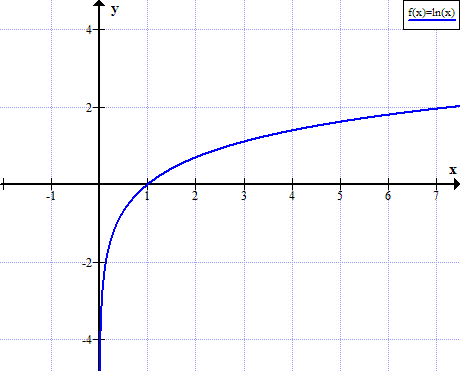
\includegraphics[width=80mm]{log.png}
\caption{Log Function}
\end{figure}
The Log function has a domain and an image that ranges from 0 to $\infty$.
It is possible to see that when the argument of the function tends to zero, the limit tends to -$\infty$, 
and when the argument tends to +$\infty$, the limit also tends to +$\infty$.

% Formula 
\subsection*{Formula}
\begin{equation}
    \min_{G} \max_{D} V(D, G) = \mathbb{E}_{x \sim p_{\text{data}}(x)}[\log D(x)] 
\end{equation}
\[
+ \mathbb{E}_{z \sim p_z(z)}[\log(1 - D(G(z)))]
\]
\begin{itemize}
    \item $D(x)$: the Discriminator as output layer use the Sigmoid function which map the data in a
    range from 0 to 1 .
    \item $G(x)$: the Generator instead as output layer use the Tanh function which map the data in a
    range from -$\infty$ to $\infty$ .
\end{itemize}

Therefore, based on these outputs and the behavior of the log function, it is possible to understand why 
the generator is minimized and the discriminator is maximized in the formula.
\\\\
So in detail the log function of the first expected value must have as arguments elements between 0 and 1 at most 
(output of D), therefore the first part of the equation, trying to maximize D, sees mainly negative values and at 
most equal to 0. \\
At the same time, the second equation with the second expected value calculates the difference between [ 1 - D(G(z)) ] 
, and since the argument of D tends to -infinity and we are simultaneously trying to maximize D and minimize G, 
the difference will result in a value between 0 and 1 (always positive).
Therefore, the limit of the logarithm as it approaches 0 will be equal to -$\infty$, 
while if the argument is 1, then the result is zero. \\
It's also possible to maximize G and use the log( [ D(G(z)) ] ) equation instead of log( [ 1 - D(G(z)) ] ) and 
obtain the same result . 


\subsection*{
    Text Encoder and Image Encoder via CLIP
}
To obtain a vector representation of text descriptions the main paper used the approch 
of Reed in 2006 using Deep convolutional and simmetric architecture based on both 
images a its corresponding text description . \\
The main idea in to have a dataset (Training set ) composed of N elements : 
\\
$ \{(v_n, t_n, y_n) : n = 1, ..., N\} $
\\
in which :
\begin{itemize}
    \item $ v_n $: correspond to the N images
    \item $ t_n $: correspond to the N text description
    \item $ y_n $: correspond to the class label ( usually there are more than two usually M )
\end{itemize}

First of all the paper define the classifier for both images and text description :
\begin{equation}
    f_v(v) = \arg \max_{y \in \mathcal{Y}} \mathbb{E}_{t \sim \mathcal{T}(y)} [\phi(v)^T \varphi(t)]
\end{equation}
    
\begin{equation}
    f_t(t) = \arg \max_{y \in \mathcal{Y}} \mathbb{E}_{v \sim \mathcal{V}(y)} [\phi(v)^T \varphi(t)]
\end{equation}

So in the first equation from all the possible class labels ($y$) we are trying to find the one that maximize the correlation between 
the input image and all the text descriptions on all the classes . \\
To do it we compute the multiplication between the encoded version of the input image $v$ and the current text description ($t$)
related to the current class . \\
In practice $\phi(v)$ and $\varphi(t )$ return a vector and we compute the similarity via a vector multiplication that return a scalar .\\ 
To compute the expected value in practice we compute the mean of all the scalar that we obtain from 
this multiplication on the specific class ($y$) .\\
In the second equation the formula is similar but on the input text description ($t$) .
The main idea was that an encoded description should have an higher compatibility 
with the images related to its class and so obtain higher value 

\begin{itemize}
    \item $\mathcal{Y}$: Set of the classes in which the images are divided .
    \item $\mathcal{T}(y)$: Set of the text description related to the $y$ class .
    \item $\mathcal{V}(y)$: Set of the images related to the $y$ class .
    \item $f_v(v)$: Classifier based on the images which return the class with higher compatibility with the image $v$
    \item $f_t(t)$: Classifier based on text description which return the class with higher compatibility with the description $t$
    \item $\phi(v)$: Image Encoder rappresentation on $v$ already trained on different dataset which return a vector (es. Obtained via CNN ).
    \item $\varphi(t)$: Text Encoder rappresentation on $t$ already trained on different dataset which return a vector (es. Obtained via CNN or LSTM).
    \item $\Delta$: Hinge or 0-1 loss for classification defined in which if the argument is higher than 0 it return 0 or 1 otherwise
    \item $\mathbb{E}_{t \sim \mathcal{T}(y)}$: Expected value in which $t$ correspond to all the text description related at the $y$ class .
    \item $\mathbb{E}_{v \sim \mathcal{V}(y)}$:  Expected value in which $v$ correspond to all the images related at the $y$ class .
\end{itemize}

Hinge or 0-1 Loss in this case is:

\begin{equation}
    \Delta( y, f(x) ) = max (0 , 1 - y * f(x) )
\end{equation}



\begin{equation}
    \varphi_{loss} = \frac{1}{N} \sum_{n=1}^{N} \Delta(y_n, f_v(v_n)) + \Delta(y_n, f_t(t_n)) 
\end{equation}

The main idea to compute the $\varphi_{loss}$ loss function was to learn the weights of 
the Text Encoder ($\varphi$) and fine-tuning it on our dataset .

During our implementation part this fine-tuning part has been done using 
the CLIP (Contrastive Language-Image Pre-Training) Text Encoder on the 
complete CUB and Flower dataset , in such a way to obtain 
relevant vector rappresentation which is composed of values that ranges 
from negative to positive values .

